\documentclass[aspectratio=169]{beamer}

\usepackage{fontspec}
\IfFontExistsTF{Times New Roman}{\setmainfont{Times New Roman}}{\setmainfont{TeX Gyre Termes}}
\IfFontExistsTF{Arial}{\setsansfont{Arial}}{\setsansfont{TeX Gyre Heros}}
\IfFontExistsTF{Menlo}{\setmonofont{Menlo}}{\setmonofont{DejaVu Sans Mono}}
\usepackage[russian]{babel}
\usepackage{booktabs}
\usepackage{array}
\usepackage{graphicx}
\graphicspath{{./}{presentation/}}
\usepackage{tikz}
\usepackage{hyperref}
\usetikzlibrary{arrows.meta, positioning, shapes.geometric}

\usetheme{Madrid}
\usecolortheme{default}
\definecolor{SandBackground}{HTML}{F7E9DA}
\definecolor{SoftSand}{HTML}{EBD4C0}
\definecolor{DustyRose}{HTML}{C98291}
\definecolor{DeepRose}{HTML}{7A3E48}
\definecolor{WarmText}{HTML}{2F2526}
\setbeamercolor{normal text}{fg=WarmText,bg=SandBackground}
\setbeamercolor{structure}{fg=DeepRose}
\setbeamercolor{title}{fg=white,bg=DeepRose}
\setbeamercolor{subtitle}{fg=SoftSand}
\setbeamercolor{author}{fg=WarmText}
\setbeamercolor{institute}{fg=WarmText}
\setbeamercolor{date}{fg=WarmText}
\setbeamercolor{frametitle}{fg=white,bg=DustyRose}
\setbeamercolor{framesubtitle}{fg=SoftSand}
\setbeamercolor{palette primary}{fg=white,bg=DeepRose}
\setbeamercolor{palette secondary}{fg=white,bg=DustyRose}
\setbeamercolor{palette tertiary}{fg=WarmText,bg=SoftSand}
\setbeamercolor{palette quaternary}{fg=white,bg=DeepRose}
\setbeamercolor{titlelike}{fg=white,bg=DustyRose}
\setbeamercolor{block title}{fg=white,bg=DustyRose}
\setbeamercolor{block body}{fg=WarmText,bg=SoftSand!65!white}
\setbeamercolor{itemize item}{fg=DeepRose}
\setbeamercolor{itemize subitem}{fg=DustyRose}
\setbeamercolor{enumerate item}{fg=DeepRose}
\setbeamercolor{section in toc}{fg=DeepRose}
\setbeamercolor{subsection in toc}{fg=DustyRose}
\setbeamercolor{caption name}{fg=DeepRose}
\setbeamertemplate{navigation symbols}{}
\setbeamertemplate{itemize items}[circle]

\title[Навигация по линиям]{Навигация и картография робота по линиям}
\subtitle{Восстановление 2D-траектории робота по видео и IMU}
\author[В. Перепечаев, А. Адамов, Т. Вязовик]{Перепечаев Виктор, Артур Адамов, Тимофей Вязовик \\ Ментор: Николай Кузнецов}
\institute[МФТИ]{Московский физико-технический институт}
\date{\today}

\newcommand{\project}{Навигация и картография робота по линиям}
\newcommand{\code}[1]{\texttt{#1}}

\begin{document}

% ============================================================
\begin{frame}
    \titlepage
\end{frame}

\begin{frame}{Содержание}
    \tableofcontents
\end{frame}

% ============================================================
\section{Команда}

\begin{frame}{Команда проекта}
    \begin{itemize}
        \item \textbf{Перепечаев Виктор}
        \item \textbf{Артур Адамов}
        \item \textbf{Тимофей Вязовик} --- работает над статьёй (область работы полностью отдельная от нашей).
        \item \textbf{Ментор:} Николай Кузнецов
    \end{itemize}

    \vspace{0.6em}
    Распределение ролей --- смешанное: оба участника (Виктор и Артур) были ответственны за все направления (CV, IMU, алгоритмы, инфраструктура), задачи перераспределялись по ситуации.

    \vspace{0.6em}
    \small В самом начале семестра \textbf{один из участников команды отчислился}, что повлияло на распределение нагрузки и приоритизацию задач.
\end{frame}

% ============================================================
\section{Постановка проблемы}

\begin{frame}{Постановка проблемы}
    \textbf{Дано:}
    \begin{itemize}
        \item видео с двух камер ZED --- \code{Right\_cam.mp4} и \code{Left\_cam.mp4},
        \item IMU-данные (акселерометр + гироскоп),
        \item timestamps кадров видео,
        \item Kalibr-калибровки IMU и camera-IMU.
    \end{itemize}

    \vspace{0.6em}
    \textbf{Требуется:} восстановить 2D-траекторию робота $(x, y, \mathrm{yaw})$ во времени и визуализировать её.
\end{frame}

\begin{frame}{Особенности входных данных}
    \begin{itemize}
        \item Робот движется по \textbf{синей ленте} на полу.
        \item Камера ZED содержит две монокулярные секции (LEFT и RIGHT): абсолютный масштаб напрямую из одной не восстанавливается, но два независимых наблюдения позволяют его уточнить.
        \item IMU --- потребительский MEMS: gyro подходит для интегрирования yaw, accel для translation --- нет (drift $\sim t^2$).
        \item Видео и IMU имеют независимые timestamps в наносекундах --- нужна синхронизация по абсолютному времени.
    \end{itemize}
\end{frame}

% ============================================================
\section{Цель}

\begin{frame}{Цель проекта}
    \begin{block}{Цель}
        Создать воспроизводимый офлайн-пайплайн, который по записи видео и IMU строит 2D-траекторию робота.
    \end{block}
\end{frame}

% ============================================================
\section{Ресурсы и технологии}

\begin{frame}{Ресурсы и технологии}
    \begin{columns}[t]
        \begin{column}{0.48\textwidth}
            \textbf{Языки и инструменты:}
            \begin{itemize}
                \item Python 3.10--3.14
                \item \code{uv} --- менеджер зависимостей
                \item Beamer (\code{xelatex}) --- презентация
                \item Git, GitHub Actions --- CI
            \end{itemize}

            \vspace{0.4em}
            \textbf{Computer Vision:}
            \begin{itemize}
                \item OpenCV (HSV, distance transform, morphological operations)
                \item Plotly --- интерактивные HTML-графики
            \end{itemize}
        \end{column}
        \begin{column}{0.48\textwidth}
            \textbf{Sensor fusion / Math:}
            \begin{itemize}
                \item NumPy, SciPy
                \item IMU preintegration
                \item Kalibr (\code{T\_cam\_imu}, \code{timeshift\_cam\_imu}, AprilGrid)
                \item SVD, Procrustes, MAD-фильтр
            \end{itemize}

            \vspace{0.4em}
            \textbf{Качество:}
            \begin{itemize}
                \item \code{pytest}, \code{ruff}, \code{mypy}
                \item Coverage badge в CI
            \end{itemize}
        \end{column}
    \end{columns}
\end{frame}

% ============================================================
\section{Календарное планирование}

\begin{frame}{Календарное планирование}
    \small
    \begin{table}
        \begin{tabular}{>{\raggedright\arraybackslash}p{0.20\textwidth} >{\raggedright\arraybackslash}p{0.72\textwidth}}
            \toprule
            Период & Активность \\
            \midrule
            Февраль (1-я пол.) & Постановка задачи, инвентаризация данных, изучение Kalibr и формата SVO. \\
            Февраль (2-я пол.) & Калибровка камеры (обход бага Kalibr с одной камерой), отладка ZED-stack. \\
            Март (1-я пол.) & Калибровка IMU через AprilGrid, синхронизация времени видео и IMU. \\
            Март (2-я пол.) & Базовое интегрирование yaw, gravity alignment, миграция инфраструктуры на \code{uv}. \\
            Апрель (1-я пол.) & Реализация \code{tape\_line}: HSV-маска, centerline, базовая интеграция позы. \\
            Апрель (2-я пол.) & Офлайн-сглаживание, адаптивный confidence, variable speed correction. \\
            Май (1-я пол.) & Loop averaging: нарезка по кругам, alignment, quality gate, ручные \code{--lap-bounds}. \\
            Май (2-я пол.) & Использование второй камеры, fusion LEFT + RIGHT, тесты, CI, документация. \\
            \bottomrule
        \end{tabular}
    \end{table}
\end{frame}

% ============================================================
\section{Реализация}

\begin{frame}{Общая схема пайплайна}
    \centering
    \begin{tikzpicture}[
        node distance=0.30cm,
        block/.style={rectangle, draw, fill=blue!10, text width=0.85\textwidth, align=center, minimum height=0.55cm, font=\small},
        arrow/.style={-{Stealth[length=2mm]}, thick}
    ]
        \node[block] (a) {Чтение конфига + CLI overrides + Kalibr YAML};
        \node[block, below=of a] (b) {Загрузка IMU CSV, timestamps кадров; нормализация времени};
        \node[block, below=of b] (c) {Калибровка IMU: \code{R\_cam\_imu}, gravity align, yaw-bias};
        \node[block, below=of c] (d) {Автонастройка HSV $\rightarrow$ детекция синей ленты};
        \node[block, below=of d] (e) {Интегрирование позы $\rightarrow$ raw\_traj $\rightarrow$ smoothed\_traj};
        \node[block, below=of e] (f) {Loop averaging + quality gate $\rightarrow$ круг};
        \node[block, below=of f] (g) {Слияние кругов LEFT + RIGHT $\rightarrow$ итоговый круг};
        \node[block, below=of g] (h) {CSV + Plotly HTML};

        \draw[arrow] (a) -- (b);
        \draw[arrow] (b) -- (c);
        \draw[arrow] (c) -- (d);
        \draw[arrow] (d) -- (e);
        \draw[arrow] (e) -- (f);
        \draw[arrow] (f) -- (g);
        \draw[arrow] (g) -- (h);
    \end{tikzpicture}
\end{frame}

\begin{frame}{Измерение шумов IMU (Allan deviation)}
    \begin{columns}[c]
        \begin{column}{0.46\textwidth}
            Перед Kalibr-калибровкой IMU был измерен \textbf{Allan deviation} акселерометра по осям X, Y, Z.

            \vspace{0.5em}
            По графику оцениваются:
            \begin{itemize}
                \item \textbf{White noise} (наклон $-1/2$) --- $\sigma_a$ плотность шума;
                \item \textbf{Random walk} (наклон $+1/2$) --- $\sigma_{a, bias}$.
            \end{itemize}

            \vspace{0.5em}
            Эти параметры записываются в \code{imu-imu\_calibration.yaml} и используются IMU preintegration.
        \end{column}
        \begin{column}{0.52\textwidth}
            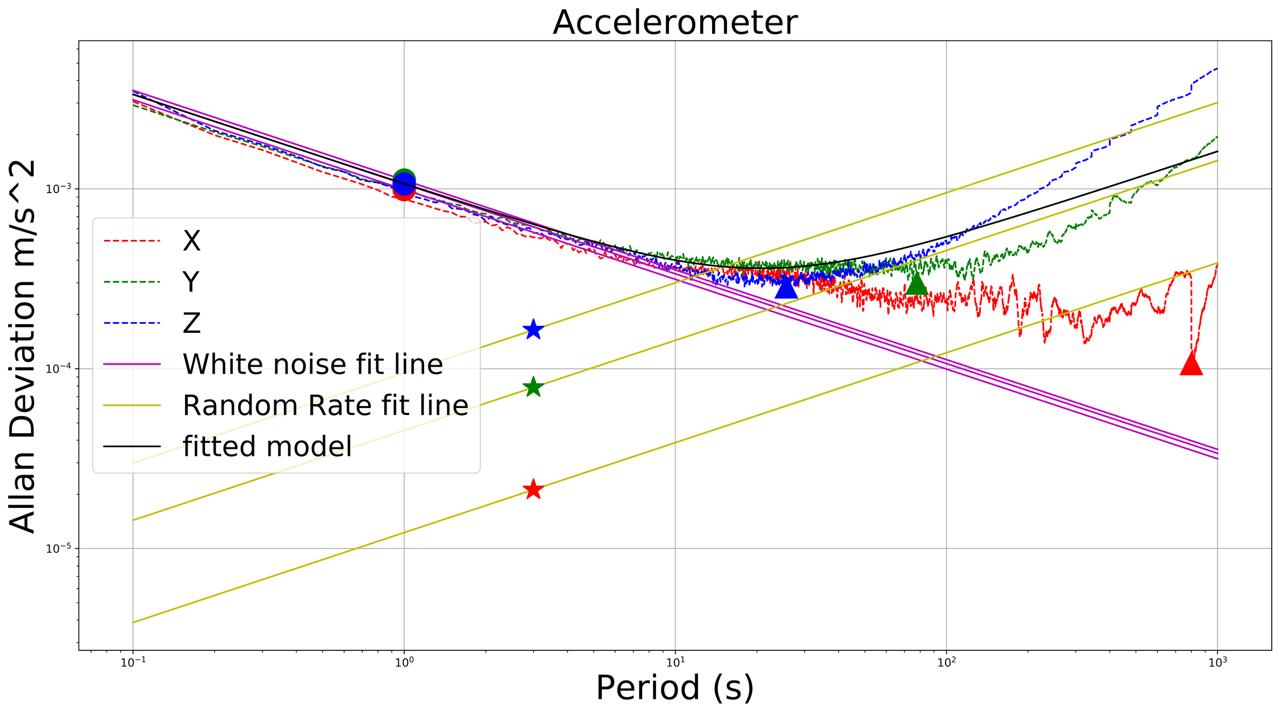
\includegraphics[width=\linewidth]{../images/image1.png}
        \end{column}
    \end{columns}
\end{frame}

\begin{frame}{Режим \code{tape\_line}}
    \begin{columns}[t]
        \begin{column}{0.48\textwidth}
            \textbf{Детекция ленты:}
            \begin{itemize}
                \item Resize $\to$ HSV $\to$ \code{inRange}
                \item Largest connected component
                \item Median blur + morphological close
                \item Distance transform $\to$ centerline
            \end{itemize}

            \textbf{Confidence по кадру:}
            \begin{itemize}
                \item Число точек centerline
                \item Вертикальный span
                \item Площадь маски
                \item Валидность угла
            \end{itemize}
        \end{column}
        \begin{column}{0.48\textwidth}
            \textbf{Офлайн-сглаживание:}
            \begin{itemize}
                \item Адаптивный порог confidence по распределению
                \item Centered weighted MA по \code{angle\_rad} и \code{bottom\_x}
                \item Окно задаётся в секундах, не кадрах
            \end{itemize}

            \textbf{Интеграция позы:}
            \begin{itemize}
                \item yaw $\leftarrow$ yaw + $\Delta$yaw$_{IMU}$ + correction
                \item $\Delta x, \Delta y$ = $v \cdot s_i \cdot dt \cdot (\cos, \sin)$
                \item lateral correction по \code{bottom\_x}
            \end{itemize}
        \end{column}
    \end{columns}
\end{frame}

\begin{frame}{Усреднение кругов (loop averaging)}
    \begin{itemize}
        \item Оценка периода круга по визуальным дескрипторам кадров.
        \item Нарезка на круги: автоматически (anchor / по периоду) или вручную через \code{--lap-bounds}.
        \item Выравнивание кругов через rigid Procrustes (SVD без масштаба).
        \item Отброс плохих кругов: MAD-фильтр выбросов + quality gate по RMSE.
        \item Итоговый круг --- лучший представитель со сглаживанием.
    \end{itemize}
\end{frame}

\begin{frame}{Слияние LEFT + RIGHT}
    \begin{columns}[c]
        \begin{column}{0.46\textwidth}
            \begin{itemize}
                \item Каждая камера строит свой круг независимо.
                \item LEFT выравнивается к RIGHT (rigid Procrustes + phase search).
                \item Итог --- точечное среднее двух кругов.
                \item Два независимых наблюдения снижают variance ошибки.
            \end{itemize}
        \end{column}
        \begin{column}{0.52\textwidth}
            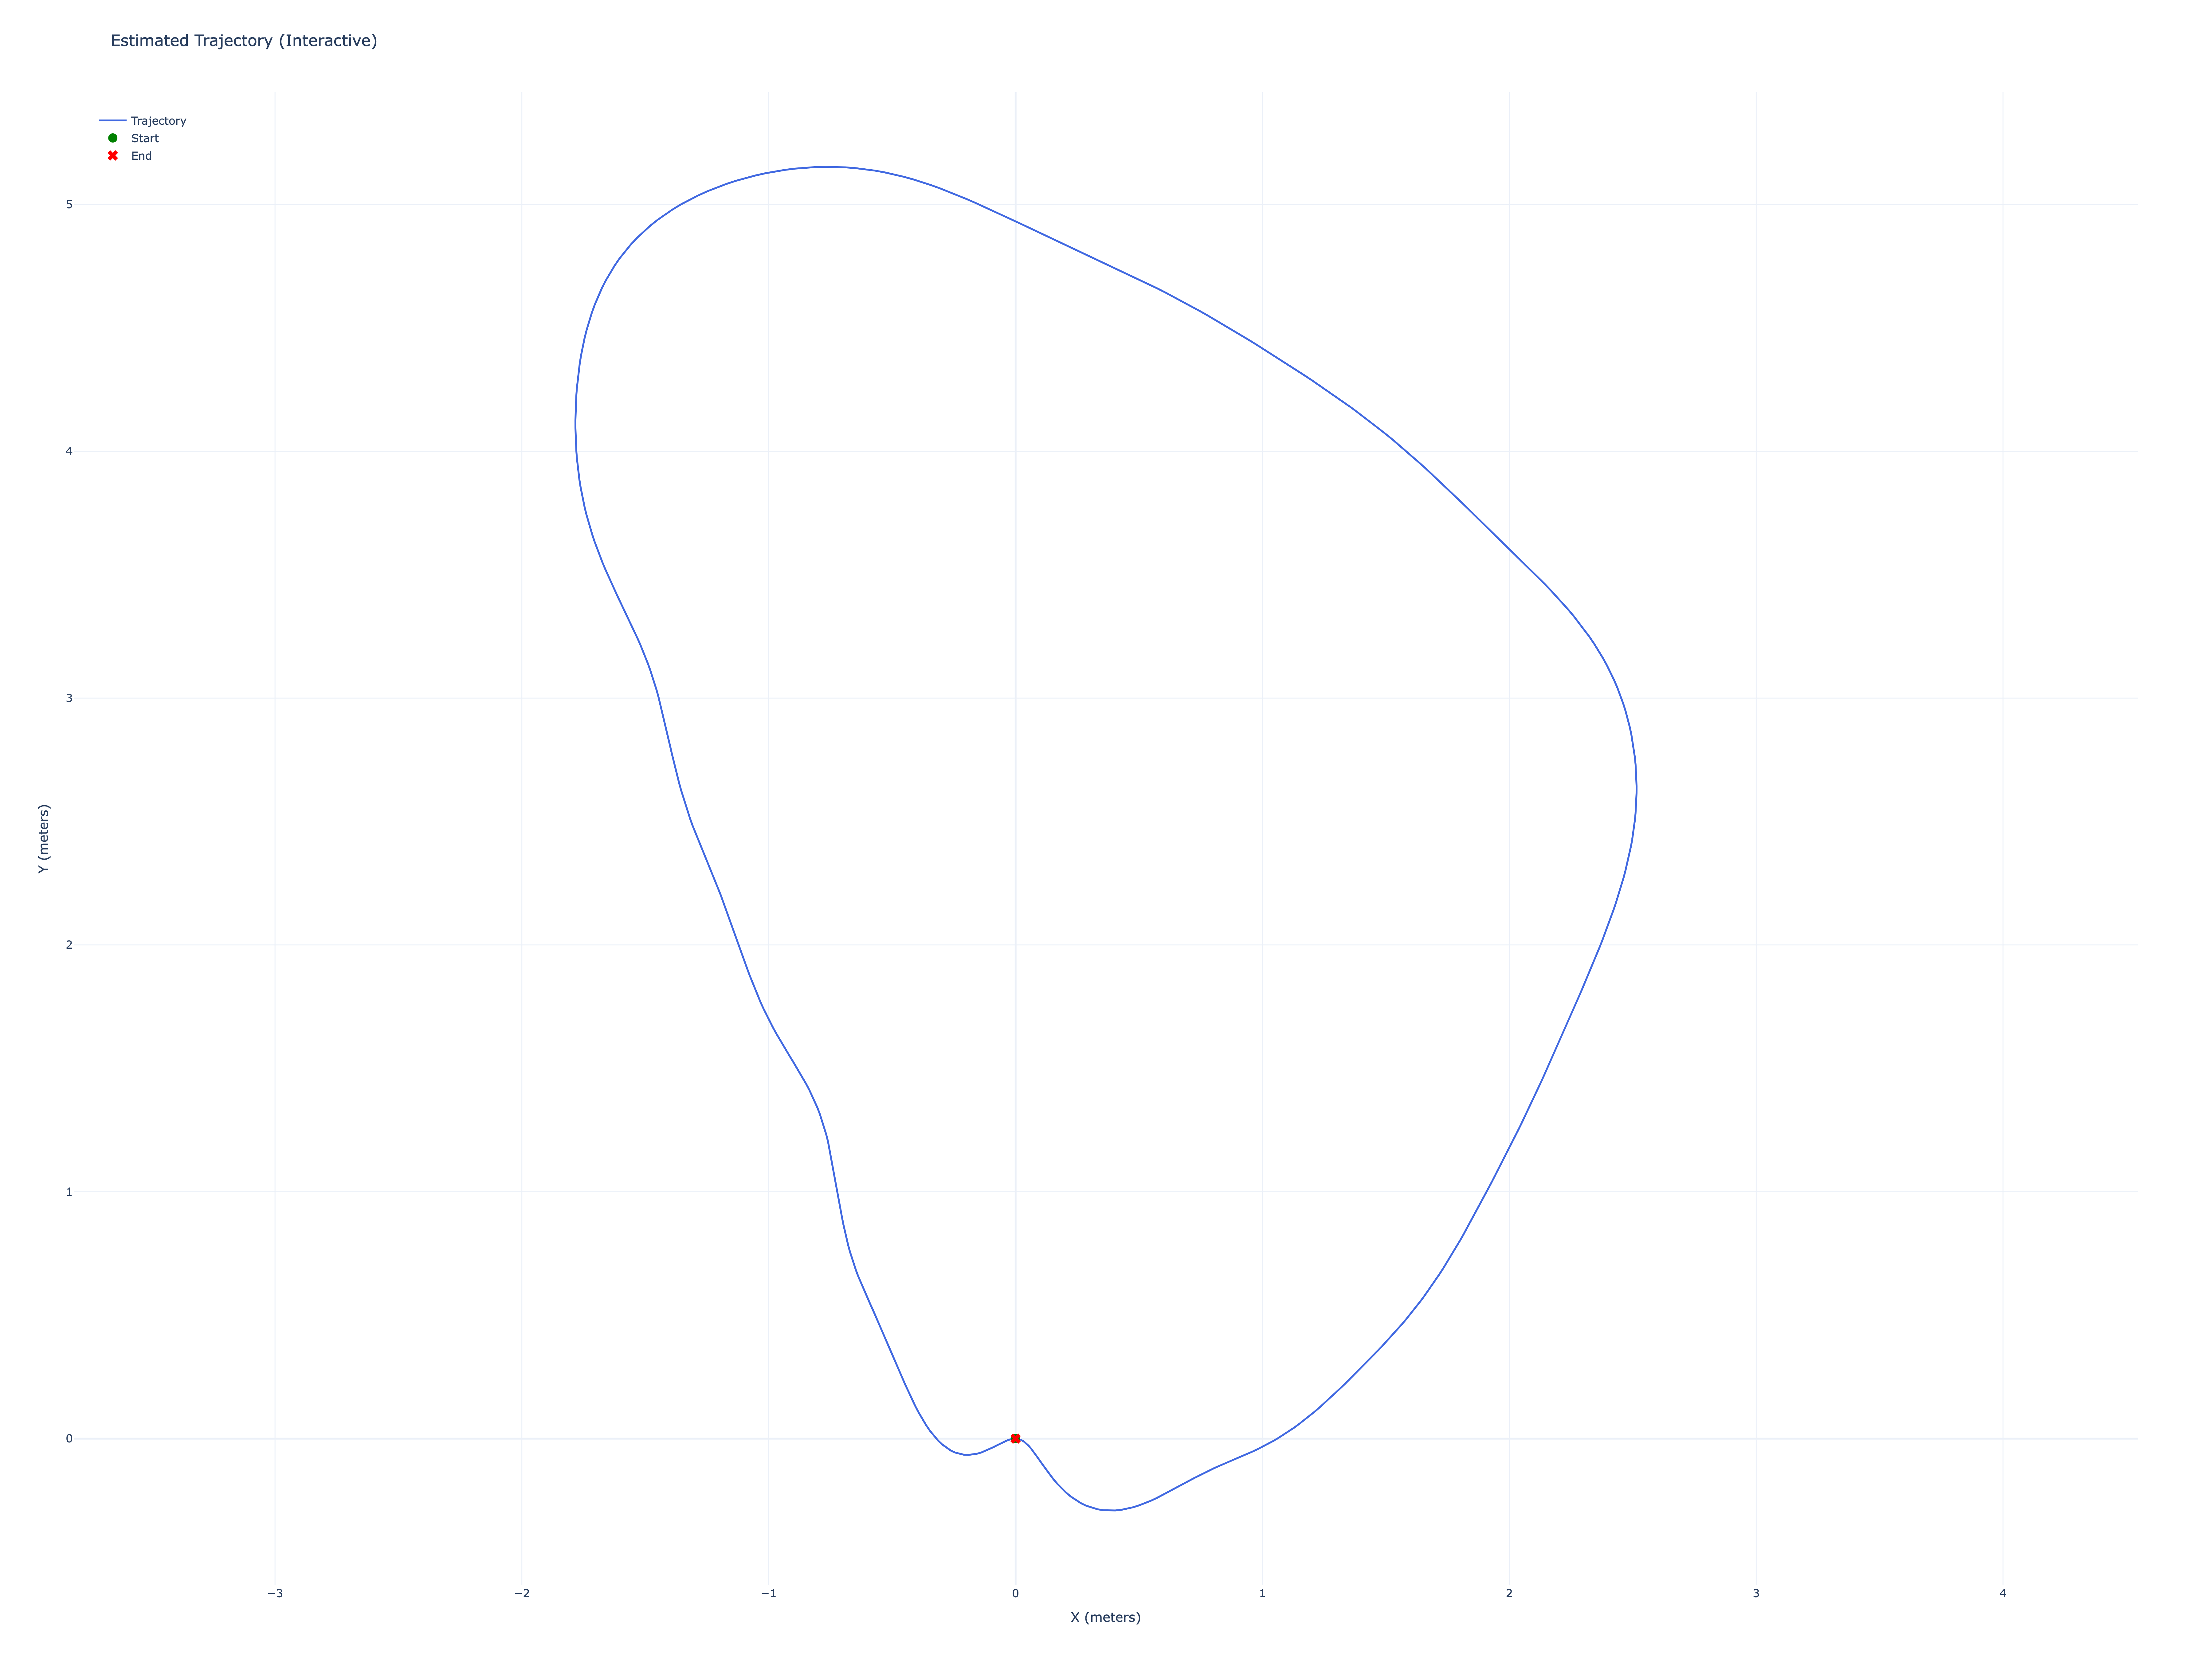
\includegraphics[width=\linewidth]{../images/image2.png}
            \vspace{-0.3em}
            \begin{center}\tiny Итоговая траектория --- усреднение LEFT и RIGHT.\end{center}
        \end{column}
    \end{columns}
\end{frame}

% ============================================================
\section{Проблемы и их решения}

\begin{frame}{Проблема 1: третий круг идёт против часовой стрелки}
    \textbf{Симптом:} 1-й и 2-й круги CW, 3-й --- CCW; автодетекция направление обхода не различает.

    \vspace{0.4em}
    \textbf{Решение:} CLI-флаг \code{--lap-bounds} для явного указания границ кругов.
\end{frame}

\begin{frame}{Проблема 2: робот стоит первые 11 секунд}
    \textbf{Симптом:} стационарный старт сбивает anchor-search; найденные границы кругов сдвигаются относительно реальных.

    \vspace{0.4em}
    \textbf{Решение:} ручные \code{--lap-bounds} с явным указанием начала первого круга в 11 с.
\end{frame}

\begin{frame}{Проблема 3: IMU translation drift}
    \textbf{Симптом:} двойное интегрирование accel даёт ошибку $\sim t^2$ --- через один круг сопоставимо с самим кругом.

    \vspace{0.4em}
    \textbf{Решение:} yaw из IMU (один интеграл, drift медленный), translation --- из априорного \code{forward\_speed\_mps} с variable-speed correction.
\end{frame}

\begin{frame}[fragile]{Проблема 4: Kalibr не работает с одной камерой}
    \textbf{Симптом:} intrinsic-калибровка падает с Python-исключением --- библиотека рассчитана на multi-camera setup.

    \vspace{0.4em}
    \textbf{Источник:} \href{https://github.com/ethz-asl/kalibr/issues/364}{ethz-asl/kalibr \#364}; проверка связности графа в \code{MulticamGraph.py}.

    \vspace{0.4em}
    \textbf{Решение} (из community):
    \begin{verbatim}
sed -i 's/return self.G.adhesion()/return True/g' \
  .../kalibr_camera_calibration/MulticamGraph.py
    \end{verbatim}
\end{frame}

\begin{frame}{Проблема 5: IMU-калибровка и инфраструктура}
    \begin{itemize}
        \item Kalibr + AprilGrid: требовалось физически вращать робота по всем осям, чтобы оценить параметры IMU.
        \item Ни у кого в команде не было ноутбука с NVIDIA GPU --- часть инструментов (SVO2 от ZED) требует CUDA.
        \item Привлекали сторонних людей: Роберт Вахненко предоставлял свой ноутбук для конвертации SVO2.
    \end{itemize}
\end{frame}

% ============================================================
\section{Сравнительные результаты}

\begin{frame}{Сравнение вариантов прогона (одна камера vs две)}
    \small
    \begin{table}
        \begin{tabular}{>{\raggedright\arraybackslash}p{0.28\textwidth} c c c}
            \toprule
            Вариант & Длина (м) & Bbox (м) & Aspect \\
            \midrule
            RIGHT auto (3 круга, full) & 11,32 & $3{,}42 \times 3{,}80$ & 1,11 \\
            RIGHT \code{--lap-bounds}  & 12,70 & $3{,}04 \times 4{,}57$ & 1,51 \\
            LEFT \code{--lap-bounds}   & 10,89 & $3{,}00 \times 4{,}10$ & 1,37 \\
            \textbf{FUSED LEFT + RIGHT} & \textbf{11,22} & $\mathbf{2{,}93 \times 4{,}27}$ & \textbf{1,46} \\
            \bottomrule
        \end{tabular}
    \end{table}

    \vspace{0.5em}
    \textbf{Качество выравнивания LEFT $\to$ RIGHT:}
    \begin{itemize}
        \item Mean residual: \textbf{0,34 м} ($\sim$8\% от bbox)
        \item Median: 0,28 м, p95: 0,78 м
        \item Reflection не нужна --- обе камеры дают траекторию в одной ориентации
    \end{itemize}
\end{frame}

% ============================================================
\section{Итоги}

\begin{frame}{Итоги}
    \begin{block}{Что получено}
        \begin{itemize}
            \item Воспроизводимый офлайн-пайплайн \project{} с использованием двух камер ZED.
            \item Замкнутый круг по записи с несколькими повторениями, усреднённый по LEFT + RIGHT.
            \item CI с тестами, типизацией и линтером; coverage badge.
        \end{itemize}
    \end{block}

    \begin{block}{Чему научились}
        \begin{itemize}
            \item Sensor fusion в условиях ограниченного бюджета (monocular + MEMS IMU).
            \item Робастные методы (MAD, quality gates, адаптивные пороги).
            \item Инженерные практики: \code{uv}, CI, отладка библиотек уровня Kalibr.
        \end{itemize}
    \end{block}
\end{frame}

% ============================================================
\section{Дальнейшее развитие}

\begin{frame}{Направления дальнейшего развития}
    \begin{columns}[t]
        \begin{column}{0.32\textwidth}
            \textbf{Алгоритм:}
            \begin{itemize}
                \item Pose graph optimization для коррекции дрейфа.
                \item Bundle adjustment с camera intrinsics.
            \end{itemize}
        \end{column}
        \begin{column}{0.32\textwidth}
            \textbf{Сенсоры:}
            \begin{itemize}
                \item Stereo / depth $\to$ метрический масштаб без \code{forward\_speed}.
                \item Wheel odometry как дополнительный prior.
            \end{itemize}
        \end{column}
        \begin{column}{0.32\textwidth}
            \textbf{Функционал:}
            \begin{itemize}
                \item Чтение стрелочных символов на поле.
                \item Сценарии «следуй за объектом X».
                \item Тестирование в разных условиях освещения.
                \item Интеграция с прошлогодним ROS-стеком.
            \end{itemize}
        \end{column}
    \end{columns}
\end{frame}

\begin{frame}
    \begin{center}
        \vspace{1.5cm}
        {\Huge Спасибо за внимание!}
    \end{center}
\end{frame}

\end{document}
